\section{Introdução}

\subsection{Contextualização}

\begin{frame}{Foguetes de sondagem}
    \begin{itemize}[<+->]
        \item Foguete de lançamento terrestre sub-orbital
        \item A Sequência de operação consiste em \visible<+->{lançamento}\visible<+->{, abertura de paraquedas}\visible<+->{, pouso}\visible<+->{ e localização}
        \item Em alguns casos, o lançamento é realizado onde não há sinal de internet
        \item Mas mesmo nesses casos, é possível haver o sinal da telemetria de bordo
    \end{itemize}
    % % \begin{center}
\begin{tikzpicture}

    % Variables


    \coordinate (bottomleft) at (-0.5,-0.5);
    \coordinate (topright) at (10.5,5);

    \def\coordref[#1](#2){%

        \coordinate(sysref) at (#2);

        \draw[#1, -latex] (sysref) ++(-0.4,-0.3) -- ++(0.9,0) node[midway, below]{$x$};
        \draw[#1, -latex] (sysref) ++(-0.3,-0.4) -- ++(0,0.9) node[midway, left]{$y$};
        \draw[#1, -latex] \centerarc(sysref)(-90:180:0.25);
        \draw[#1] (sysref) node{$+$}
    }

    % \draw[Red,dashed] (bottomleft) rectangle (topright);
    \clip (bottomleft) rectangle (topright);

    \coordinate (O) at (0,0);

    % \draw [help lines, dashed] (bottomleft) grid (topright); % desenha grid
    % \draw [red] (O) node[draw,cross out] {}; % marca pont(0,0)

    % \draw[Red] (4,2)
    %     node[draw, thick, shape=foguete, fill=cmyk_R!25, scale=4] {}
    %     node[draw, circle, inner sep=2pt] {}
    % ;

    % \shade[inner color=yellow,outer color=white] (6,0) rectangle +(2,1);

    % \draw
    %     (-0.5,0) -- (10.5,0)
    % ;


    \coordinate (left) at (-0.5,0);
    \coordinate (right) at (10.5,0);
    \coordinate (middle) at ($(left)!0.5!(right)$);
    \draw[thin, Black!50, path fading=west] (left) -- (middle);
    \draw[thin, Black!50, path fading=east] (middle) -- (right);
    % \shade[draw, inner color=Green!10,outer color=Red] (-0.5,0) -- (10.5,3);


    \draw[cmyk_K] (0,0) node[draw, shape=foguete, fill=cmyk_R, anchor=south, rotate=0] {};

    \draw[cmyk_K] (0.5,2) node[OrangeRed, rotate=170, anchor=south, inner sep=-2.5pt, xshift=0.25pt] {\Fire} node[draw, shape=foguete, fill=cmyk_R, anchor=south, rotate=-10] {};

    \draw[cmyk_K] (5,4) node[draw, shape=foguete, fill=cmyk_R, anchor=south, rotate=-95] {};

    \draw[cmyk_K] (9,0) node[draw, shape=foguete, fill=cmyk_R, anchor=east, rotate=-90] {};



    \begin{pgfonlayer}{background}    % select the background layer
        \clip (bottomleft) rectangle (10.5,0);
        \shade[inner color=SaddleBrown!50,outer color=White] (bottomleft) rectangle (10.5,0.5);
    \end{pgfonlayer}


\end{tikzpicture}
% \end{center}
    \begin{center}
        \visible<+->{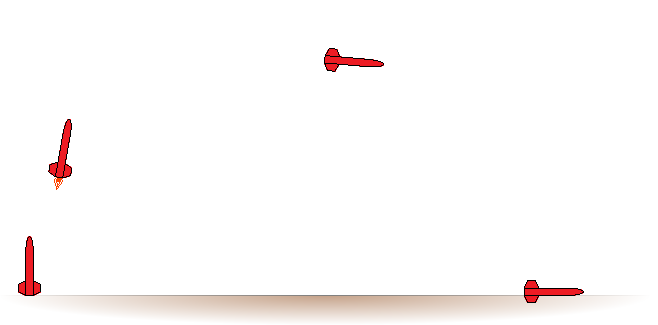
\includegraphics{../pictures/conops.pdf}}
    \end{center}
\end{frame}

\subsection{Objetivos}
\begin{frame}{Objetivos}
    \begin{itemize}[<+->]
        % \item Construir um equipamento capaz de localizar o foguete
        \item Utilizar métodos de AoA para determinar direção de origem do sinal
        \item Comparar a performance com um sistema semelhante baseado em GPS
        % \item Fazer um sistema portátil, para ser levado em campo
    \end{itemize}
\end{frame}
